\documentclass[
]{jss}

\usepackage[utf8]{inputenc}

\providecommand{\tightlist}{%
  \setlength{\itemsep}{0pt}\setlength{\parskip}{0pt}}

\author{
H. Sherry Zhang\\Monash University \And Dianne Cook\\Monash University
\AND Ursula Laa\\University of Natural Resources and Life Sciences
\AND Nicolas Langrené\\CSIRO Data61 \AND Patricia
Menéndez\\Monash University \AND
}
\title{\pkg{cubble}: An R Package for Structuring Spatio-temporal Data}

\Plainauthor{H. Sherry Zhang, Dianne Cook, Ursula Laa, Nicolas
Langrené, Patricia Menéndez}
\Plaintitle{cubble: An R Package for Structuring Spatio-temporal Data}

\Abstract{
The abstract of the article.
}

\Keywords{spatio-temporal data, \proglang{R}}
\Plainkeywords{spatio-temporal data, R}

%% publication information
%% \Volume{50}
%% \Issue{9}
%% \Month{June}
%% \Year{2012}
%% \Submitdate{}
%% \Acceptdate{2012-06-04}

\Address{
          }

% Pandoc citation processing

% Pandoc header

\usepackage{amsmath}

\begin{document}

\newpage

\hypertarget{introduction}{%
\section{Introduction}\label{introduction}}

\textbf{Motivation}

In spatio-temporal data analysis, there's a need for a new
spato-temporal data structure. The requirement for such a tool is
necessary given the ubiquity of spatio-temporal data in the wild.
Example of this includes house price of a city or county, climate
station data from the government,

\textbf{Existing packages}

Many data structures have been proposed for spatial and temporal data,
but not many for spatio-temporal data. One of the reason could be the
inherent different levels of information make it inefficient to store in
the same table. \texttt{spacetime}\citep{spacetime} proposed four
space-time layouts: Full grid (STF), sparse grid(STS), irregular (STI),
and trajectory (STT) based on underlying spatial structure \texttt{sp}
\citep{sp} and temporal structure \texttt{xts}\citep{xts}.
\texttt{spatstat} \citep{spatstat} implements a \texttt{ppp} class for
point pattern data. More recent package \texttt{stars} \citep{stars}
uses a spatiotemporal array to store the data and the array structure
has its influence from \texttt{cubelyr} \citep{cubelyr}, a dplyr data
cube backend. \newline

\textbf{Our new data structure for spatio-temporal data}

In this paper, a new spatio-temporal data structure, \texttt{cubble}, is
introduced. \texttt{cubble} implements a relational data structure that
splits the data into its spatial and temporal component. With this
structure, users can separately manipulate the spaital or temporal
component of the data while keep the two dimension linked. The software
is available from the Comprehensive R Archive Network (CRAN) at {[}CRAN
link{]}. \newline

\textbf{Section division}

The rest of the paper will be divided as follows: Section 2 reviews the
existing data structure for spatio, temporal, and spatio-temporal data.
Section 3 presents a new data structure for spatio-temporal data:
cubble. Then the paper introduces the workflow of data manipulation and
visualisation with the cubble structure in Section 4. Section 5 gives
some examples on how common spatial and temporal manipulations are
performed with cubble and how static and interactive visualisation help
to understand climate and {[}\ldots{]} data. \newline

\textbf{Criteria of a data structure we want}

With recent development in the R community, \texttt{sf} \citep{sf} and
\texttt{tsibble}\citep{tsibble} have replaced \texttt{sp} and
\texttt{xts} to be the convention structure for spatial and temporal
data. One reason for their popularity is its integration with tidyverse
ecosystem, making them intuitive and easy to adopt. For spatio-temporal
data, we hope to build a data structure has the following features:

\begin{enumerate}
\def\labelenumi{\arabic{enumi})}
\tightlist
\item
  A data structure that handles spatial and temporal dimension in a
  relational structure. This derives from the 3rd tidy data principal.
\item
  An intuitive and easy to use interface that fits into the tidyverse
  ecosystem, and
\item
  Compatibility with the latest spatial and temporal data structure.
  This would give users the flexibility to use the work in existing
  packages.
\end{enumerate}

\textbf{Spatio-temporal data + examples}\\
Spatio-temporal data record changes of variables in spatially separated
regions across time. In this article, we consider spatio-temporal vector
data, which are recorded in a fixed interval. Examples of this type of
data include the house price of a city or county, climate measures from
weather stations in a country, and river level data from electronic
gauges \textcolor{red}{more examples here}. \newline

\textbf{point to common feature: spatial level variables + time level
variables relates to Table 13 in Tidy data paper}\\
Usually, this type of spatio-temporal data does not necessarily come in
as a single table. Tidy data principle \citep{tidydata} prescribes each
type of observational unit to form a table. This would suggest two
tables to store the data, one for spatial-level and one for
temporal-level. The Table 13 in \citet{tidydata} presents a structure
like this and the author argues the lack of tools to work with
relational data like such. \newline

\textbf{My proposal}\\
Recent software development in R has proposed several relational data
structure: \texttt{tidygraph}\citep{tidygraph} for graph manipulation,
\texttt{dm} \citep{dm} for relational data model, while spatio-temporal
data could benefit from having its own relational data structure that
identifies the essential spati0-temporal element: site identifier, time
identifier, geographic coordinates. \newline

\newpage

\hypertarget{lit-review}{%
\section{Existing data structure for spatio and temporal
data}\label{lit-review}}

\newpage

\hypertarget{cubble-data-structure}{%
\section{Cubble data structure}\label{cubble-data-structure}}

\hypertarget{spatio-temporal-data-in-the-wild}{%
\subsection{Spatio-temporal data in the
wild}\label{spatio-temporal-data-in-the-wild}}

Spatio-temporal data don't usually come to the analysts in various
forms. Figure \ref{fig:cubble-diagram} groups them into four categories.
Despite whichever form the data is in, all the forms have a group
identifier, \texttt{key}, a time column, \texttt{t}, and variables that
either various across group, i.e.~\texttt{lon}, \texttt{lat}, \(C_s\),
or across time, i.e.~\(V_t\). These identifiers will be the building
blocks for the data structure introduced below.

\begin{CodeChunk}
\begin{figure}

{\centering 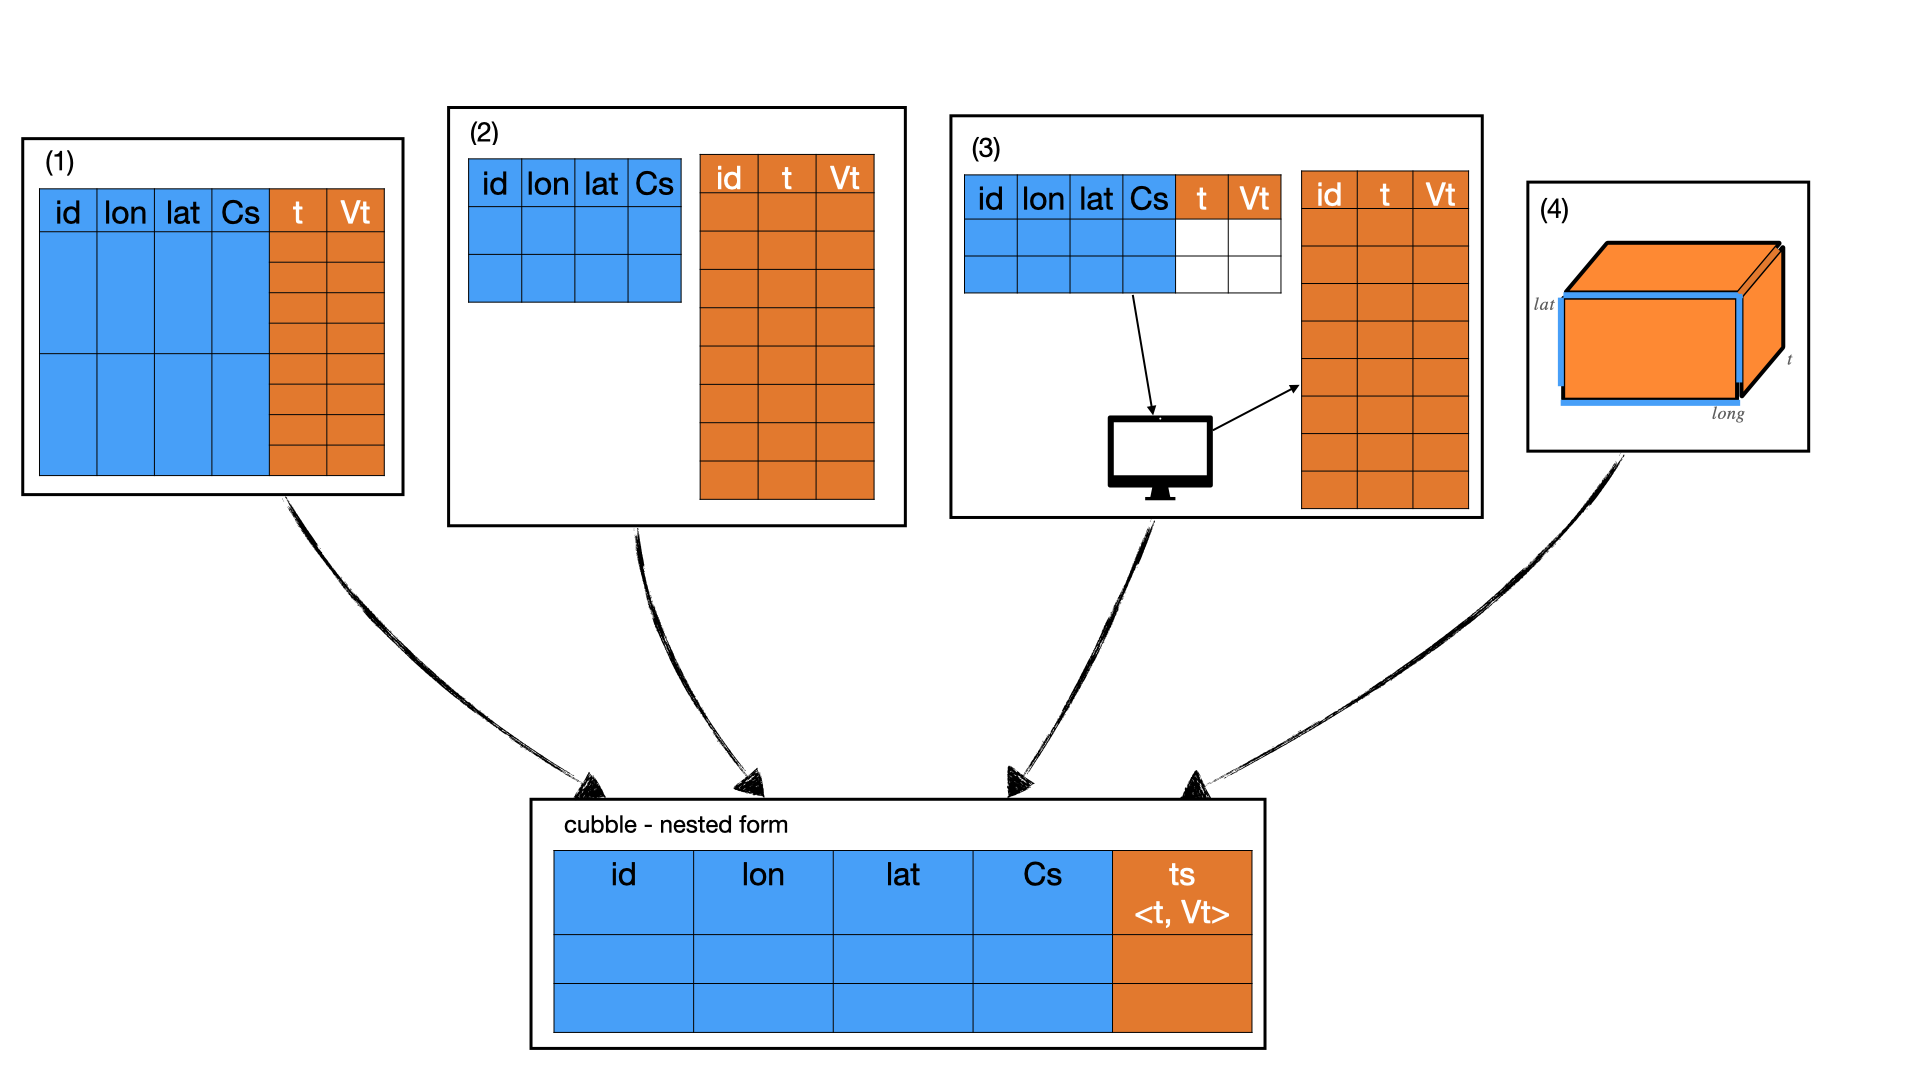
\includegraphics[width=1\linewidth,height=0.15\textheight]{/Users/sherryzhang/Documents/research/paper-cubble/figures/input-formats/input-formats.001} 

}

\caption[Illustration of incoming data formats for spatio-temporal data]{Illustration of incoming data formats for spatio-temporal data. (1) Data comes in as a single table; (2) Separate tables for spatial and temporal variables; (3) A single table with all the parameters used to query the database and a separate table for queried data; and (4) Cubical data in array or NetCDF format.}\label{fig:cubble-diagram}
\end{figure}
\end{CodeChunk}

\hypertarget{a-new-data-structure-cubble}{%
\subsection{A new data structure:
cubble}\label{a-new-data-structure-cubble}}

A cubble, in essence, wires the spatial and temporal dimension into a
single object while provides two forms for manipulation each dimension
separately.

In the nest form, Figure \ref{fig:def-cubble}a), a cubble:

\begin{itemize}
\tightlist
\item
  defines each group in a row,
\item
  displays the group-related variables in columns, and
\item
  nests all the time-related variables into a column called \texttt{ts}.
\end{itemize}

In the long form, Figure \ref{fig:def-cubble}b), a cubble:

\begin{itemize}
\tightlist
\item
  defines the combination of group and timestamp as a row
\item
  displays time-related variables, along with the group identifier in
  columns, and
\item
  stores group-related variables as a attributes called
  \texttt{spatial}.
\end{itemize}

\begin{CodeChunk}
\begin{figure}

{\centering 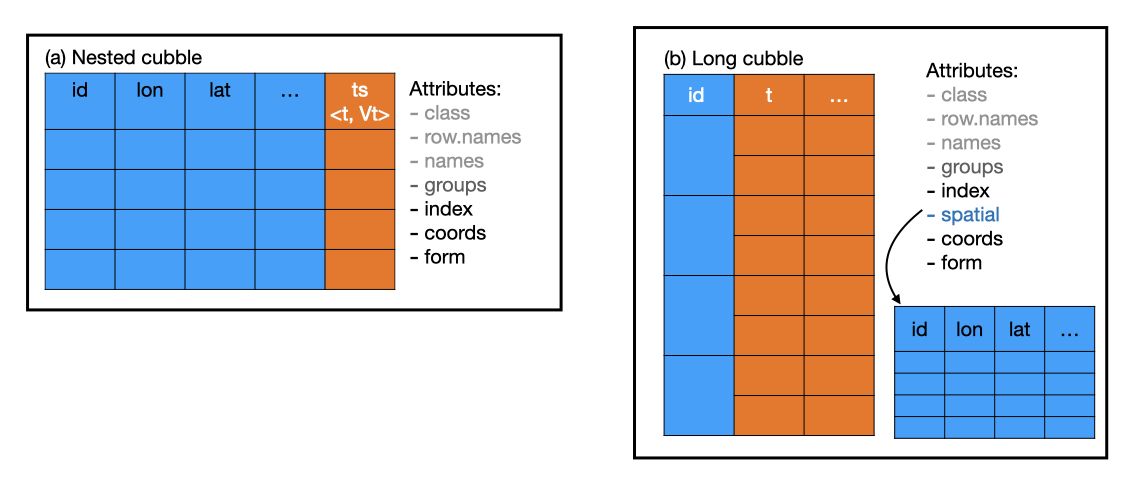
\includegraphics[width=1\linewidth,height=0.3\textheight]{/Users/sherryzhang/Documents/research/paper-cubble/figures/def-cubble/def-cubble.001} 

}

\caption[Illustration of nested and long cubble]{Illustration of nested and long cubble.}\label{fig:def-cubble}
\end{figure}
\end{CodeChunk}

\newpage

\hypertarget{create-a-cubble-in-the-nested-form}{%
\subsection{Create a cubble in the nested
form}\label{create-a-cubble-in-the-nested-form}}

To create a cubble, you can use \texttt{as\_cubble} with proper supply
of \texttt{key}, \texttt{index}, and \texttt{coords}. {[}\texttt{key}
defines whether a variable is spatial or temperal by looking at whether
it varies across \texttt{key}. For example, \texttt{lat} is a spatial
variable since for one \texttt{id} there's only one \texttt{lat} value.
\texttt{index} and \texttt{coords} prescribes the temporal index and
spaital coordinates used in the data. These are common variables that
should present in the point pattern spatio-temporal data.{]} The cubble
created by default is in the nested form. \newline

\begin{CodeChunk}
\begin{CodeInput}
R> (cubble_nested <- climate_flat %>% 
+   as_cubble(key = id, index = date, coords = c("long", "lat")))
\end{CodeInput}
\begin{CodeOutput}
# cubble:   id [5]: nested form
# bbox:     [115.97, -32.94, 133.55, -12.42]- check gap on long and lat
# temporal: date [date], prcp [dbl], tmax [dbl], tmin [dbl]
  id            lat  long  elev name           wmo_id ts                
  <chr>       <dbl> <dbl> <dbl> <chr>           <dbl> <list>            
1 ASN00009021 -31.9  116.  15.4 perth airport   94610 <tibble [366 x 4]>
2 ASN00010311 -31.9  117. 179   york            94623 <tibble [366 x 4]>
3 ASN00010614 -32.9  117. 338   narrogin        94627 <tibble [366 x 4]>
4 ASN00014015 -12.4  131.  30.4 darwin airport  94120 <tibble [366 x 4]>
5 ASN00015131 -17.6  134. 220   elliott         94236 <tibble [366 x 4]>
\end{CodeOutput}
\end{CodeChunk}

In the \texttt{cubble} header, you can read the key variable + number,
bbox, and also the name of variable nested in the \texttt{ts} column.
Here in this example, the temporal variables are precipitation,
\texttt{prcp}, maximum temporature, \texttt{tmax}, and minimum
temperature, \texttt{tmin}.

In this structure, the nested form is suitable for manipulating the
spatial dimension of the data and this would include manipulating
variables that 1) are inherently spatial and 2) summarise the temporal
variables by \texttt{key}. Under the hood, the nested cubble is built on
top of the rowwise dataframe (\texttt{rowwise\_df}). This is design to
simplify the code when working with the temporal variables - they are
nested into the list-column \texttt{ts}.

\hypertarget{stretch-a-nested-cubble-into-the-long-form}{%
\subsection{Stretch a nested cubble into the long
form}\label{stretch-a-nested-cubble-into-the-long-form}}

The verb \texttt{stretch()} switch the cubble from the nested form into
a long form. Under the hood, it first extracts the spatial variables
into a separate tibble to store in the attribute \texttt{spatial} and
then unnests the \texttt{ts} column to show the temporal content:

\begin{CodeChunk}
\begin{CodeInput}
R> (cubble_long <- cubble_nested %>% stretch(ts))
\end{CodeInput}
\begin{CodeOutput}
# cubble:  date, id [5]: long form
# bbox:    [115.97, -32.94, 133.55, -12.42]- check gap on long and lat
# spatial: lat [dbl], long [dbl], elev [dbl], name [chr], wmo_id [dbl]
   id          date        prcp  tmax  tmin
   <chr>       <date>     <dbl> <dbl> <dbl>
 1 ASN00009021 2020-01-01     0  31.9  15.3
 2 ASN00009021 2020-01-02     0  24.9  16.4
 3 ASN00009021 2020-01-03     6  23.2  13  
 4 ASN00009021 2020-01-04     0  28.4  12.4
 5 ASN00009021 2020-01-05     0  35.3  11.6
 6 ASN00009021 2020-01-06     0  34.8  13.1
 7 ASN00009021 2020-01-07     0  32.8  15.1
 8 ASN00009021 2020-01-08     0  30.4  17.4
 9 ASN00009021 2020-01-09     0  28.7  17.3
10 ASN00009021 2020-01-10     0  32.6  15.8
# ... with 1,820 more rows
\end{CodeOutput}
\end{CodeChunk}

Notice here that the third line in the header is changed to reflect the
spatial variables stored. This is a format suitable for computing
time-wise variables.

\hypertarget{tamp-a-long-cubble-back-to-the-nested-form}{%
\subsection{Tamp a long cubble back to the nested
form}\label{tamp-a-long-cubble-back-to-the-nested-form}}

Manipulation on the spatial and temporal dimension can be an iterative
process. Many times, we may decide to go back to the nested form after
some temporal manipulation. The verb to switch a long cubble back to the
nested form is \texttt{tamp()}:

\begin{CodeChunk}
\begin{CodeInput}
R> (cubble_back <- cubble_long %>% tamp())
\end{CodeInput}
\begin{CodeOutput}
# cubble:   id [5]: nested form
# bbox:     [115.97, -32.94, 133.55, -12.42]- check gap on long and lat
# temporal: date [date], prcp [dbl], tmax [dbl], tmin [dbl]
  id            lat  long  elev name           wmo_id ts                
  <chr>       <dbl> <dbl> <dbl> <chr>           <dbl> <list>            
1 ASN00009021 -31.9  116.  15.4 perth airport   94610 <tibble [366 x 4]>
2 ASN00010311 -31.9  117. 179   york            94623 <tibble [366 x 4]>
3 ASN00010614 -32.9  117. 338   narrogin        94627 <tibble [366 x 4]>
4 ASN00014015 -12.4  131.  30.4 darwin airport  94120 <tibble [366 x 4]>
5 ASN00015131 -17.6  134. 220   elliott         94236 <tibble [366 x 4]>
\end{CodeOutput}
\end{CodeChunk}

\hypertarget{migrate-spatial-variables-to-a-long-cubble}{%
\subsection{Migrate spatial variables to a long
cubble}\label{migrate-spatial-variables-to-a-long-cubble}}

As an output to be supplied to further visualisation or modelling,
analysts would usually like the spatial and temporal variables to be in
the same table. \texttt{migrate()} moves the spatial variables in the
attribute \texttt{spatial} into the long form cubble.

\begin{CodeChunk}
\begin{CodeInput}
R> (cubble_long %>% migrate(long, lat))
\end{CodeInput}
\begin{CodeOutput}
# cubble:  date, id [5]: long form
# bbox:    [115.97, -32.94, 133.55, -12.42]- check gap on long and lat
# spatial: lat [dbl], long [dbl], elev [dbl], name [chr], wmo_id [dbl]
   id          date        prcp  tmax  tmin  long   lat
   <chr>       <date>     <dbl> <dbl> <dbl> <dbl> <dbl>
 1 ASN00009021 2020-01-01     0  31.9  15.3  116. -31.9
 2 ASN00009021 2020-01-02     0  24.9  16.4  116. -31.9
 3 ASN00009021 2020-01-03     6  23.2  13    116. -31.9
 4 ASN00009021 2020-01-04     0  28.4  12.4  116. -31.9
 5 ASN00009021 2020-01-05     0  35.3  11.6  116. -31.9
 6 ASN00009021 2020-01-06     0  34.8  13.1  116. -31.9
 7 ASN00009021 2020-01-07     0  32.8  15.1  116. -31.9
 8 ASN00009021 2020-01-08     0  30.4  17.4  116. -31.9
 9 ASN00009021 2020-01-09     0  28.7  17.3  116. -31.9
10 ASN00009021 2020-01-10     0  32.6  15.8  116. -31.9
# ... with 1,820 more rows
\end{CodeOutput}
\end{CodeChunk}

\hypertarget{support-on-hierarchical-structure}{%
\subsection{Support on hierarchical
structure}\label{support-on-hierarchical-structure}}

\texttt{switch\_key()}

\hypertarget{integrating-into-a-tidy-workflow}{%
\subsection{Integrating into a tidy
workflow}\label{integrating-into-a-tidy-workflow}}

Building from an underlying \texttt{tbl\_df} structure, it is natural to
implement methods available in \texttt{dplyr} to \texttt{cubble}.
Supported methods in the \texttt{cubble} with \texttt{dplyr} generics
includes: \texttt{mutate}, \texttt{filter}, \texttt{summarise},
\texttt{select}, \texttt{arrange}, \texttt{rename}, \texttt{left\_join},
\texttt{group\_by}, \texttt{ungroup}, and the slice family
(\texttt{slice\_head}, \texttt{slice\_tail}, \texttt{slice\_sample},
\texttt{slice\_min} and \texttt{slice\_max})
\textcolor{red}{into a table}.

\texttt{cubble} is also compatible with \texttt{tsibble} in the sense
that the original list-column can be a \texttt{tbl\_ts} object.
Duplicates and gaps shoudl be first checked before structuring the data
into a cubble. If the input data is a \texttt{tsibble} object, the long
form cubble is also a \texttt{tsibble} where users can directly apply
time series operations.

\newpage

\hypertarget{examples}{%
\section{Examples}\label{examples}}

\hypertarget{australia-precipitation-pattern-in-2020}{%
\subsection{Australia precipitation pattern in
2020}\label{australia-precipitation-pattern-in-2020}}

Forming a cubble + basic tidyverse verbs - Vig 2 Aggregation - Vig 4

\hypertarget{matching-precipitation-and-river-level-in-victria-water-gauges}{%
\subsection{Matching precipitation and river level in Victria water
gauges}\label{matching-precipitation-and-river-level-in-victria-water-gauges}}

Matching - Vig 3

\hypertarget{conclusion}{%
\section{Conclusion}\label{conclusion}}

\newpage

\hypertarget{old-stuff}{%
\section{Old stuff}\label{old-stuff}}

Many spatial and spatio-temporal data structures have been developed by
the R-spatial team for both raster and vector spatial data. For vector
spatial data, which is the focus of this paper, \texttt{sf}
\citep{pebesma2018simple} represents spatial vector information with
simple features: points, lines, polygons and their multiples. Various
\texttt{st\_} function are designed to manipulate these features based
on their geometric relationships. For spatio-temporal data,
\texttt{stars} \citep{stars} can represent both raster and vector data
using multi-dimensional array. However, the underlying array structure
can be difficult to operate for data analysts who are more familiar with
a flat 2D data frame structure used by the tidyverse ecosystem.

In the temporal aspect, the \texttt{tsibble} \citep{tsibbles} structure
and its tidyverts ecosystem have provided a {[}\ldots{} {]} workflow to
work with temporal data. In a tsibble structure, temporal data is
characterised by \texttt{index} and \texttt{key} where \texttt{index} is
the temporal identifier and \texttt{key} is the identifier for multiple
series, which could be used as a spatio identifier. However, a tsibble
object, by construction, always requires the \texttt{index} in its
structure. This makes it less appealing for spatio-temporal data since
the output of calculated spatio-specific variables (i.e.~features of
each series) don't have the time dimension. Analysts will either need to
have an additional step to join this output to the original tsibble or
operate with variables stored in two separate objects. In addition, the
long form structure of a tsibble object means spatio variables
(i.e.~longitude, latitude, and features of each series if joined back to
the tsibble) of each spatio identifier will be repetitively recorded at
each timestamp. This repetition is unnecessary and would inflate the
object size for long series.

\hypertarget{a-new-data-structure-for-spatio-temporal-data}{%
\section{A new data structure for spatio-temporal
data}\label{a-new-data-structure-for-spatio-temporal-data}}

\textbf{The main difficulty and challenge}\\
The main difficulty in visualising this type of data is to show
information in both space and time dimension with the proper level of
details without information overflow. This would sometimes require
aggregating the time dimension into the proper level or slicing the data
into a reasonable number of subset for display. In this sense, a data
structure that regulates the manipulation spatio-temporal data will
benefit the analysis workflow. While many implementations focus on
manipulating and visualising pure spatial or temporal data, there are
not sufficient tools to deal with spatio-temporal data. The purpose of
this paper is to introduce a spatio-temporal vector data structure for
data analysis in R.

To work with spatio-temporal data, analysts can choose to either work
separately on each dimension or join the two sets together, however,
each approach has its own problem: While is is natural to work
separately on each sheet (since spatial and temporal operations usually
don't overlap), analysts will need to manually keep the other data frame
up to date. For example, the following pseudo code illustrates the
scenario where once the spatial dataset is filtered for those within
Victoria, the temporal dataset needs to be manually updated to reflect
this spatial filter.

\begin{CodeChunk}
\begin{CodeInput}
R> spatial_new <- spatial %>% filter(SITES_IN_VICTORIA)
R> temporal_new <- temporal %>% filter(id %in% spatial_new$id)
\end{CodeInput}
\end{CodeChunk}

If analysts choose to join the spatial and temporal data together, the
joined dataset could be too large since each spatial variable will be
repeated at each time stamp for each site. Also, recordings of the site
ID from different data sources can be slightly different from each
other, causing a painful checking and cleaning of site IDs before the
join.

\newpage

\hypertarget{create-a-cubble}{%
\section{Create a cubble}\label{create-a-cubble}}

The creation of a cubble requires the site identifier (\texttt{key}), as
well as the spatial (\texttt{coords}) and temporal (\texttt{index})
identifier. \texttt{climate\_flat} is already a tibble and it uses
\texttt{id} to identify each station, \texttt{date} as the time
identifier, and \texttt{c(long,\ lat)} as the spatial identifier. To
create a cubble for this data, use:

\begin{CodeChunk}
\begin{CodeInput}
R> climate_flat %>% as_cubble(key = id, index = date, coords = c(long, lat))
\end{CodeInput}
\begin{CodeOutput}
# cubble:   id [5]: nested form
# bbox:     [115.97, -32.94, 133.55, -12.42]- check gap on long and lat
# temporal: date [date], prcp [dbl], tmax [dbl], tmin [dbl]
  id            lat  long  elev name           wmo_id ts                
  <chr>       <dbl> <dbl> <dbl> <chr>           <dbl> <list>            
1 ASN00009021 -31.9  116.  15.4 perth airport   94610 <tibble [366 x 4]>
2 ASN00010311 -31.9  117. 179   york            94623 <tibble [366 x 4]>
3 ASN00010614 -32.9  117. 338   narrogin        94627 <tibble [366 x 4]>
4 ASN00014015 -12.4  131.  30.4 darwin airport  94120 <tibble [366 x 4]>
5 ASN00015131 -17.6  134. 220   elliott         94236 <tibble [366 x 4]>
\end{CodeOutput}
\end{CodeChunk}

Most of the time, spatio-temporal data doesn't come into this form and
analysts need to query the climate variables based on station metadata.
\textcolor{red}{This is also a problem illustrated in Section 3.5 in @tidydata. Here we provide a structured way to query this data based on the row-wise operator and nested list.}
For this type of task, one can structure a metadata into a tibble and
use row-wise operator to query the climate variables into a nested list.
As an example here we demonstrate the workflow to find the 5 closest
stations to Melbourne. We first create a station data frame with the 5
target stations.

\begin{CodeChunk}
\begin{CodeOutput}
# A tibble: 5 x 8
  id            lat  long  elev name                 wmo_id  dist city     
  <chr>       <dbl> <dbl> <dbl> <chr>                 <dbl> <dbl> <chr>    
1 ASN00086038 -37.7  145.  78.4 essendon airport      95866  10.8 melbourne
2 ASN00086282 -37.7  145. 113.  melbourne airport     94866  20.1 melbourne
3 ASN00086077 -38.0  145.  12.1 moorabbin airport     94870  21.9 melbourne
4 ASN00088162 -37.4  145. 528.  wallan (kilmore gap)  94860  48.1 melbourne
5 ASN00087113 -38.0  144.  10.6 avalon airport        94854  48.8 melbourne
\end{CodeOutput}
\end{CodeChunk}

We can query the climate information into a nested list named
\texttt{ts} for each station with the \texttt{rowwise()} operator. To
create a cubble, supply the same identifiers as with the first example.

\begin{CodeChunk}
\begin{CodeInput}
R> sydmel_climate <- stations %>%
+   rowwise() %>%
+   mutate(ts = list(meteo_pull_monitors(id,
+                                        date_min = "2020-01-01",
+                                        date_max = "2020-12-31",
+                                        var = c("PRCP", "TMAX", "TMIN")) %>%
+                      select(-id))) %>%
+   as_cubble(key = id, index = date, coords = c(long, lat))
\end{CodeInput}
\end{CodeChunk}

\begin{CodeChunk}
\begin{CodeOutput}
# cubble:   id [5]: nested form
# bbox:     [144.47, -38.03, 145.1, -37.38]
# temporal: date [date], prcp [dbl], tmax [dbl], tmin [dbl]
  id            lat  long  elev name                 wmo_id  dist city   ts     
  <chr>       <dbl> <dbl> <dbl> <chr>                 <dbl> <dbl> <chr>  <list> 
1 ASN00086038 -37.7  145.  78.4 essendon airport      95866  10.8 melbo~ <tibbl~
2 ASN00086282 -37.7  145. 113.  melbourne airport     94866  20.1 melbo~ <tibbl~
3 ASN00086077 -38.0  145.  12.1 moorabbin airport     94870  21.9 melbo~ <tibbl~
4 ASN00088162 -37.4  145. 528.  wallan (kilmore gap)  94860  48.1 melbo~ <tibbl~
5 ASN00087113 -38.0  144.  10.6 avalon airport        94854  48.8 melbo~ <tibbl~
\end{CodeOutput}
\end{CodeChunk}

Below are the how the nested and long form look like for Australia
climate data, which records daily precipitation, maximum and minimum
temperature for 55 stations across Australia from 2015- 2020. Notice
that each station forms a group in both forms and specifically, the
nested and long form have a underlying \texttt{rowwise\_df} and
\texttt{grouped\_df} respectively.

With a cubic framework on mind, different types of manipulation with
cubble can be thought of as slicing the cube in various way. The table
below shows how some \texttt{dplyr} verbs are mapped into the operation
in a cubble. With the existing grouping on the station, additional
groupping can be added with \texttt{group\_by} and removed with
\texttt{ungrouped}. {[}talk about why it is useful{]}

\newpage

\hypertarget{cubble-operations}{%
\subsection{Cubble operations}\label{cubble-operations}}

\begin{CodeChunk}
\begin{figure}

{\centering 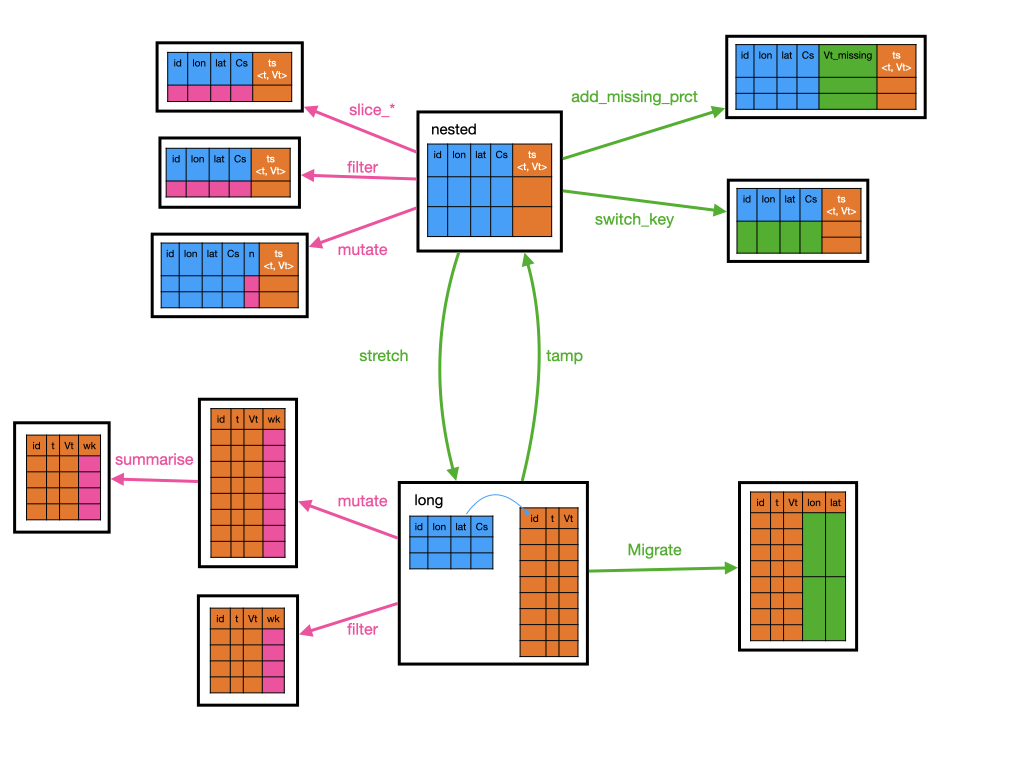
\includegraphics[width=0.9\linewidth,height=0.5\textheight]{/Users/sherryzhang/Documents/research/paper-cubble/figures/cubble-operations/cubble-operations.001} 

}

\caption[Cubble operations]{Cubble operations}\label{fig:cubble-operations}
\end{figure}
\end{CodeChunk}

\hypertarget{basics}{%
\subsubsection{Basics}\label{basics}}

\begin{itemize}
\tightlist
\item
  \texttt{stretch}: nest to long form
\item
  \texttt{tamp}: long to nest form
\item
  \texttt{migrate}: move selected spatial variables to the long form.
\item
  \texttt{add\_dscrb\_prct}: summary stats for missingness
\end{itemize}

dplyr compatibility:

\begin{itemize}
\tightlist
\item
  mutate, filter, summarise, select, arrange
\item
  group and ungroup: group\_by, ungroup
\item
  slice family
\end{itemize}

\hypertarget{combine-two-cubbles}{%
\subsubsection{Combine two cubbles}\label{combine-two-cubbles}}

\begin{itemize}
\tightlist
\item
  match river and weather gauges data
\item
  involve combining two cubbles
\item
  join operations combine the two together by appending more rows but
  what we really want is to bind rows.
\item
  bind rows also doesn't work since we want to bind only when there' s a
  matching????
\item
  introduce bind\_join
\end{itemize}

\hypertarget{hierarchical-structure-in-cubble}{%
\subsubsection{Hierarchical structure in
cubble}\label{hierarchical-structure-in-cubble}}

\begin{itemize}
\tightlist
\item
  hierarchical is common.
\item
  Given examples.
\item
  Essence: switch between different levels
\item
  introduce \texttt{switch\_key}
\end{itemize}

\hypertarget{examples-1}{%
\section{Examples}\label{examples-1}}

Daily climate data (prcp, tmax, and tmin) from RNOAA - lots of stations
across Australia

An exploratory data analysis questions: What's the climate profile look
like in Australia

\begin{itemize}
\tightlist
\item
  General features: Any general trend/ fluctuation in prcp, tmax, and
  tmin?
\item
  Local features: Any station stands out from the crowd?
\end{itemize}

\bibliography{references.bib}


\end{document}
